\documentclass[10pt, a4paper]{beamer}
%\documentclass{article}

%Metadaten
\title{Threat and Weakness Analysis in SimplyTag}

\subtitle{ORGADATA COMPANY, LEER}
\newcommand{\additionalsubtitle}{Data Science} 
\author{
		Manoj Selvaraju - 7025649 \\ 
		Vatsal Mahajan - 7025694\\ 
		Vijay Singh - 7025700
}

%\date{\today}
\date{January 15, 2025}

% siehe hesader.tex Zeile 10-16 zum Aktivieren der Notes
% Kommentare stehen in \notes{} und können im 2-screen-mode genutzt werden
%%%%%%
%
% $Autor: Wings $
% $Datum: 2020-01-18 11:15:45Z $
% $Pfad: githubtemplate/Template/Presentations/Template/slides/header.tex $
% $Version: 4620 $
%
%
% !TeX encoding = utf8
% !TeX root = Rename
%
%%%%%%


%Packages
\usepackage[utf8]{inputenc} %Für Umlaute, da BibLaTeX
\usepackage[english]{babel}
\usepackage{amsmath}
\usepackage{amsfonts}
\usepackage{amssymb}
\usepackage{colortbl}
\usepackage{cancel} %'\cancel{}', '\bcancel{}' und '\xcancel{}'

%%%%%%%%%2-Screen%%%%%%%%%%%%%%%%%%%%%%%%%%%%%%%%%%%%%%%%%%%%
\usepackage{pgfpages} 
%%%%Kommentiert für Beamer
%%%%Aktiv für Notes
%\setbeameroption{show notes on second screen=bottom}
%\setbeameroption{second mode text on second screen=bottom}
%%%%%%%%%%%%%%%%%%%%%%%%%%%%%%%%%%%%%%%%%%%%%%%%%%%%%%%%%%%%%

%Für Grafiken
\usepackage{tikz}
\usetikzlibrary{mindmap}
\usepackage{gnuplottex}
\usepackage{pgf}
\usepackage{colortbl} 
\usetikzlibrary{calc}
\usetikzlibrary{shapes,arrows} %Für Flowchart
\usetikzlibrary{shapes.geometric} %Für Flowchart
\usepackage{scalefnt}
\usetikzlibrary{decorations.markings} %Für => pfeile
\usetikzlibrary{calc,patterns,decorations.pathmorphing,decorations.markings}
%Für urls in Quellen
\usepackage{url}
%Für Diagramme (autotools)
%\usepackage{graphicx}
%\usepackage{graphviz}

%\usepackage[
%  backend=biber,
%  style=alphabetic,
%  sorting=ynt
%]{biblatex}

\usepackage[natbib=true,style=alphabetic,backend=bibtex,useprefix=true]{biblatex}

%Formatierungen
\mode<presentation>
\setbeamertemplate{headline} 
{%
\begin{beamercolorbox}[rounded=true, center]{bgcolor}
\begin{columns}[T]
\begin{column}{9cm}
{\color{gray}\begin{tiny}Hochschule Emden/Leer\end{tiny}} \\ 
{\color{gray}\begin{tiny}Department of Electrical Engineering and Computer Science\end{tiny}} \\ 
{\color{gray}\begin{tiny}Industrial Informatics\end{tiny}} \\
%{\color{gray}\begin{tiny}Innovationsforum MSR\end{tiny}}
\end{column}
\begin{column}{2cm}

\includegraphics[scale=0.25]{img/technik.jpg}
\end{column}
\end{columns}
\end{beamercolorbox}
 }
\insertsectionhead
\insertsubsectionhead
\usetheme{default}
\useinnertheme[shadow=true]{rounded}
\usebackgroundtemplate
{%
      \rule{0pt}{\paperheight}%
      \hspace*{\paperwidth}%
      \makebox[0pt][r]{
\includegraphics[width=\paperwidth]{img/hintergrund2.png}}
 }

\definecolor{HSELhellblau}{RGB}{138,198,203}
\definecolor{HSELblau}{RGB}{0,59,95}
\usecolortheme[named=HSELblau]{structure}
 \newcommand{\topline}{%
  \tikz[remember picture,overlay] {%
    \draw[HSELhellblau] ([yshift=-0.9cm]current page.north west)
             -- ([yshift=-0.9cm,xshift=\paperwidth]current page.north west);}}
\setbeamertemplate{section}[numbered]


\newcommand{\STANDARD}[2]
{
  \mode<presentation>%
  {%
     \begin{frame}[allowframebreaks]{#1} #2 \end{frame}
  }%
  \mode<article>
  {
    \fcolorbox{AliceBlue}%{Bisque} %{BlanchedAlmond}
    {LightGrey} %{Beige}   %{AliceBlue}
    {
      \begin{minipage}{\textwidth}{\bf #1} #2  \end{minipage}
      
      
    }%
    
    \medskip
    \hrulefill
  }
}

\newcommand{\MYNOTE}[1]
{
  \mode<presentation>%
  {%
     %\note{#1}
     \only<article>{#1}
  }%
  \mode<article>
  {
    #1
  }
}

% ------------
% sectionframe
% ------------
%
% #1  Der Name der section.
%
\newcommand{\sectionframe}[1]%
{%
	\begin{frame}
		\Huge
		\begin{center}
			#1 
		\end{center}
	\end{frame}%
}

\newcommand{\Mysection}[1]%
{%
  \section{#1}%
  
  \sectionframe{#1}%
}

\usepackage{listings}

% Farben für Syntax-Highlighting
\definecolor{dkgreen}{rgb}{0,.6,0}
\definecolor{dkblue}{rgb}{0.655,0.113,.364}
\definecolor{dkyellow}{cmyk}{0,0,.8,.3}

\definecolor{parameterc}{rgb}{.4,0,.6}
\definecolor{typec}{rgb}{0,0.525,.702}
\definecolor{stringc}{rgb}{0,.5019,.5019}
\definecolor{keywordc}{rgb}{.6549, .1137, .3647}
\definecolor{commentc}{rgb}{.5882, .5960, .5882}
\definecolor{textc}{rgb}{.2,.2,.2}

\lstdefinestyle{all}{
	alsoletter={-},
	frame=single, 	% top,frame=bottom,
	numbers=none,
	numberstyle=\tiny\color{textc},
	basicstyle=\linespread{0.9}\ttfamily\footnotesize\color{textc},
	tabsize=4,
	showstringspaces=false,
	captionpos=t,
	rulecolor=\color{lightgray!40},
	keywordstyle=\color{keywordc},
	stringstyle=\color{stringc},
	commentstyle=\color{commentc},
	breaklines=true,
	escapechar="!",
	postbreak=\mbox{\textcolor{green}{$\hookrightarrow$}\space},
}

\lstdefinestyle{bashstyle}{
	style=all,
	keywords=[2]{-y, --no-install-recommends, --allow-change-held-packages, --allow-downgrades, --fetch-keys, -n, --version, --params, -c, -i, -O, --upgrade, --no-cache-dir, --extra-index-url, --show, -s, -m},
	keywordstyle=[2]\color{parameterc},
	morekeywords = {ln,choco,pip,pip3,apt,apt-key,apt-get,apt-mark,add-apt-repository,wget,mktemp,dpkg,dpkg-query,echo,>>,rm,tegrastats, systemctl},
	deletekeywords={local,LOCAL},
}

\lstdefinestyle{pythonstyle}{
	style=all,
	morekeywords={as},
	keywords=[2]{True, False, None},
	keywordstyle=[2]\color{typec},
	alsoletter={_},
	keywords=[3]{max_workspace_size_bytes, precision_mode, maximum_cached_engines, use_calibration, optimizer, loss, input_shape, from_logits, metrics, batch_size, epochs, validation_data, activation, use_calibration, filters, kernel_size, pool_size, units},
	keywordstyle=[3]\color{parameterc},
	deletekeywords={compile,COMPILE},
}

\lstdefinestyle{inlinestyle}{
	style=all,
	breaklines        = true,
	breakatwhitespace = true,
	breakindent       = 2ex,
	escapechar        = *,
	numbers           = left,
	postbreak=,
}
\lstdefinelanguage{MyBash} {
	language = Bash,
	style=bashstyle,
}

\lstdefinelanguage{MyPython} {
	language = Python,
	style=pythonstyle,
}


\definecolor{PythonColor}{rgb}{0,0.5,1.}
\newcommand{\PYTHON}[1]{\textcolor{PythonColor}{\texttt{#1}}}
\definecolor{PythonColorHighLite}{rgb}{0.5,0,1.}
\newcommand{\PYTHONHL}[1]{\textcolor{PythonColorHighLite}{\texttt{#1}}}
\definecolor{MapleColor}{rgb}{1,0,0}
\newcommand{\MapleCommand}[1]{\textcolor{MapleColor}{\texttt{#1}}}
\definecolor{ShellColor}{rgb}{0,1,1.}
\newcommand{\SHELL}[1]{\textcolor{ShellColor}{\texttt{#1}}}
\definecolor{FileColor}{rgb}{1,0,1.}
\newcommand{\FILE}[1]{\textcolor{FileColor}{\texttt{#1}}}


%\addbibresource{Documents/MyLiterature.bib} %Import the bibliography file

\begin{document}
	

\setbeamercolor{bgcolor}{fg=black,bg=white}
\selectlanguage{English}
\setbeamertemplate{footline}{%
\vspace*{-.1cm}\hspace*{.5cm}
\scriptsize{%
%%\hspace*{1pt}\insertauthor
%%\inserttitle
\hspace{325pt}\insertframenumber/\inserttotalframenumber}
}

\STANDARD{}
{
  \titlepage
}

\MYNOTE
{
  \ldots
}



\STANDARD{Table of Content}
{
\tableofcontents
}

\MYNOTE
{
  \ldots
}

\setbeamercovered{transparent}


	    \section{Introduction}
		\begin{frame}
		\frametitle{Introduction}
		
		\begin{block}{Objective:}
			Identify and mitigate potential threats and weaknesses in Orgadata’s SimplyTag system.
		\end{block}
		
		
		\begin{block}{Background:}
			\begin{itemize}
				\item SimplyTag is a web application enabling quick access to construction-related data.
				\item Ensuring data integrity is critical to prevent exploitation by malicious actors.
			\end{itemize}
		\end{block}
		
		\begin{block}{Approach: }
			Analyze web application logs to detect suspicious activities and safeguard the system.
		\end{block}
		
		
	\end{frame}
	
	\section{Overview of Analysis}
	\begin{frame}
		\frametitle{Overview of Analysis}
		
		\begin{block}{}
			\begin{itemize}
				\item Analyzed large-scale web application logs for patterns and anomalies.
				\item Monitored HTTP status codes (e.g., 404 errors for bad requests, 200 codes for potential breaches).
				\item Traced user requests using trace IDs for activity tracking and debugging.
				\item Investigated user agents and request paths to identify malicious actors.
				\item Developed strategies to mitigate identified vulnerabilities and improve response protocols.
			\end{itemize}
		\end{block}
		
	\end{frame}
	

\section{Challenges we Faced}
\begin{frame}
	\frametitle{Challenges we Faced}
	
	\begin{columns}[T,onlytextwidth]
		% Single column for both text and image
		\column{1.0\textwidth}
		
		\begin{block}{}
			\begin{itemize}
				\item Managing and analyzing large-scale logs for meaningful insights.
				\item Distinguishing between genuine user activities and malicious attempts.
				\item Handling complex patterns in user behavior and request logs.
				%\item Ensuring timely detection and response to threats.
				%\item Adapting solutions to handle increasing system demands and traffic.
			\end{itemize}
		\end{block}
		
		% Add vertical space
		\vfill
		
		% Image placed below
		\centering
		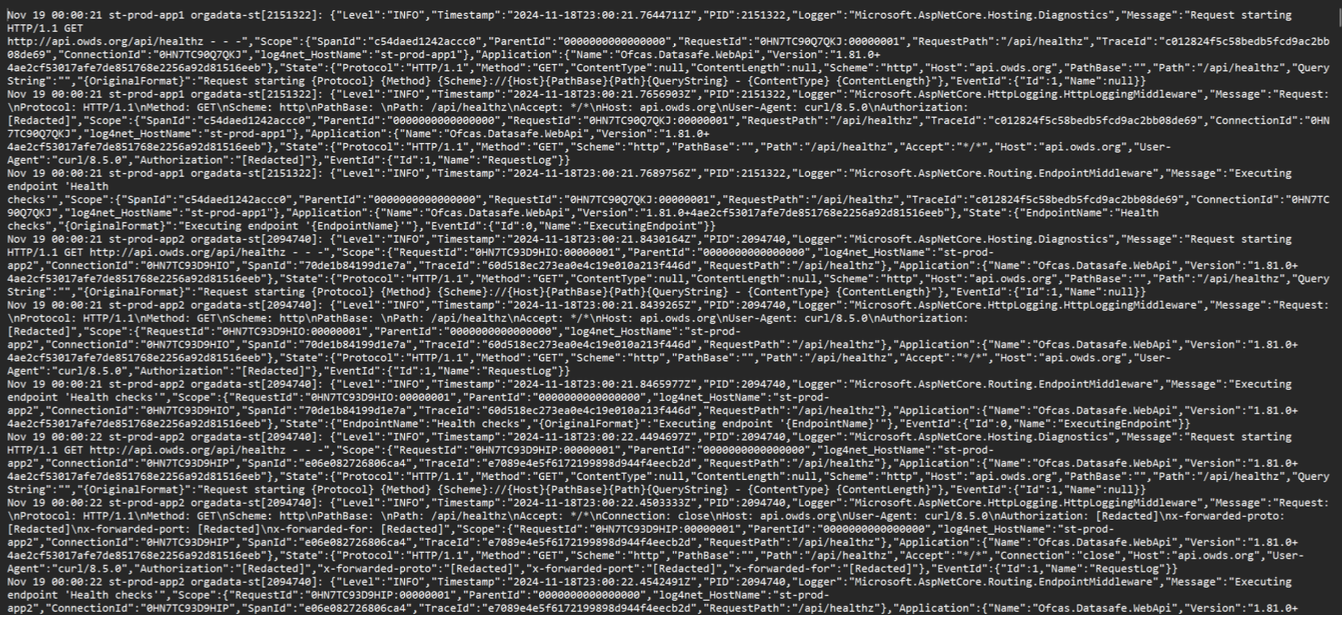
\includegraphics[width=0.8\textwidth]{images/LogSS.png} % Adjust width as needed
		
		% Image name below the image
		\vskip 0.1cm % Adds a bit of vertical space between image and text
		\centering
		\textit{Figure: Raw log data} % You can replace this with the actual name of the image
		
	\end{columns}
	
\end{frame}


	
	\section{Application Sector}
	\begin{frame}
		\frametitle{Application Sector}
		
		\begin{itemize}
			\item \textbf{Step 1: Connect the Vision Shield to the Arduino Portenta H7}
			\begin{itemize}
				\item Align the Vision Shield with the high-density connectors on the Portenta H7.
				\item Press down firmly to ensure a secure connection.
			\end{itemize}
			
			\item \textbf{Step 2: Connect the Arduino Portenta H7 to the Laptop}
			\begin{itemize}
				\item Use a USB Type-C cable to connect the Portenta H7 to your laptop.
				\item Ensure the connection is stable and the board is powered on.
			\end{itemize}
			
			\item \textbf{Step 3: Install Necessary Libraries and Dependencies}
			\begin{itemize}
				\item Open the Arduino IDE on your laptop.
				\item Navigate to the Library Manager (\texttt{Sketch} $\rightarrow$ \texttt{Include Library} $\rightarrow$ \texttt{Manage Libraries}).
				\item Install the required libraries for the Vision Shield and Portenta H7.
			\end{itemize}
			
			\item \textbf{Step 4: Verify the Hardware Connection}
			\begin{itemize}
				\item Ensure the LED on the Portenta H7 starts blinking green.
				\item If the board does not respond, double-press the reset button to enter bootloader mode.
			\end{itemize}
		\end{itemize}
		
	\end{frame}
	
	
	\section{What the Analytics is doing?}
	\begin{frame}
		\frametitle{What the Analytics is doing?}
		
		\begin{itemize}
			\item \textbf{Loading the Pre-trained AI Model}
			\begin{itemize}
				\item Obtain a pre-trained AI model optimized for object detection.
				\item Ensure the model is compatible with the resources of the Portenta H7.
			\end{itemize}
			\vspace{0.3cm}
			
			\item \textbf{Optimizing the Model for Embedded Deployment}
			\begin{itemize}
				\item Convert the model to a format that can be efficiently run on the microcontroller.
				\item Use frameworks like TensorFlow Lite for Microcontrollers.
				\item Perform quantization to reduce the model size and inference time.
			\end{itemize}
			\vspace{0.3cm}
			
			\item \textbf{Deploying the Model on the Portenta H7}
			\begin{itemize}
				\item Load the converted model onto the Portenta H7's flash memory.
				\item Utilize Arduino libraries to interface with the model.
			\end{itemize}
			\vspace{0.3cm}
			
			\item \textbf{Real-time Inference on the Portenta H7}
			\begin{itemize}
				\item Capture images from the Vision Shield's camera.
				\item Pass the images to the AI model for inference.
				\item Interpret the output to identify and classify objects in real-time.
			\end{itemize}
		\end{itemize}
	\end{frame}
	
	
	\section{Positioning Analytics in XYZ}
	\begin{frame}
		\frametitle{Positioning Analytics in XYZ}
		\begin{itemize}
			\item \textbf{Capturing Live Video Frames:}
			\begin{itemize}
				\item The Vision Shield's camera captures live video frames.
				\item Frames are continuously fed into the Portenta H7 for processing.
			\end{itemize}
			\item \textbf{Processing Frames in Real-time:}
			\begin{itemize}
				\item Each frame is processed by the AI model deployed on the Portenta H7.
				\item The model performs object detection, identifying and classifying objects in the frame.
			\end{itemize}
			\item \textbf{Annotating Detected Objects:}
			\begin{itemize}
				\item Detected objects are annotated directly on the video feed.
				\item Bounding boxes and labels are overlaid to highlight detected objects.
			\end{itemize}
			\item \textbf{Displaying Output:}
			\begin{itemize}
				\item The annotated video feed is displayed on the Vision Shield's built-in display.
				\item Real-time feedback provides immediate visual confirmation of detected objects.
			\end{itemize}
		\end{itemize}
	\end{frame}
	
	\section{Knowledge Discovery in Database (KDD) Process}
	\begin{frame}
		\frametitle{Knowledge Discovery in Database (KDD) Process}
		\begin{itemize}
			\item Live video feed from the Vision Shield's camera module.
			\item Real-time annotation of detected objects on the video feed.
			\item Accurate and efficient object detection and classification.
			\item Instant visual feedback displayed on the Vision Shield's built-in display.
			\item Potential for further customization and integration into larger systems.
		\end{itemize}
	\end{frame}
	
	
	\section{Conclusion and Future Scope}
	\begin{frame}
		\frametitle{Conclusion and Future Scope}
		
		Real-time object detection with the Arduino Portenta H7 and Vision Shield has numerous applications across various industries:
		
		\begin{itemize}
			\item \textbf{Surveillance and Security Systems:} Enhance security measures by detecting and identifying intruders or suspicious objects in real-time.
			\item \textbf{Industrial Automation and Quality Control:} Ensure product quality by identifying defects or anomalies on manufacturing lines.
			\item \textbf{Robotics and Autonomous Navigation:} Enable robots and autonomous vehicles to perceive and react to their surroundings, enhancing safety and efficiency.
			\item \textbf{Smart Home Devices and IoT Applications:} Create intelligent devices capable of recognizing and responding to human activities or environmental changes.
		\end{itemize}
		
		Real-time object detection provides valuable insights and automation capabilities in diverse fields, making it a versatile and powerful technology for modern applications.
		
	\end{frame}
	
	
	\section{Literature}
	\begin{frame}
		\frametitle{Literature}
		
		
		\begin{itemize}
			\item The project showcases the potential of AI-enabled embedded systems for real-time object detection.
			\item By leveraging the computational power of the Arduino Portenta H7 and the image processing capabilities of the Vision Shield, complex tasks like object detection can be performed efficiently and accurately in real-time.
			\item The project opens up possibilities for a wide range of applications in industries such as surveillance, industrial automation, robotics, and IoT, where real-time object detection is crucial for decision-making and automation.
		\end{itemize}
		
	\end{frame}
	

	
\STANDARD{}
{
  \begin{columns}
    \begin{column}{0.35\textwidth}
      \begin{block}{~~~~~~Thank you}
        \centering
        for your attention
      \end{block}
    \end{column}
  \end{columns}
}

\MYNOTE{Ja, \textbf{Vielen} Dank, für Ihre Aufmerksamkeit}


	
	\end{document}
	